\documentclass[a4paper, 10pt]{article}

\usepackage{listings}
\usepackage{color}
\usepackage[frenchb]{babel}
\usepackage[utf8]{inputenc}
\usepackage[T1]{fontenc}
\usepackage{lmodern}
\usepackage{graphicx}
% Numbers and units
\usepackage[squaren, Gray]{SIunits}
\usepackage{sistyle}
\usepackage[autolanguage]{numprint}
\usepackage{fullpage}
\usepackage[margin=0.7in]{geometry}
\usepackage{multirow}
\usepackage{xparse}

\newcommand\si[2]{\numprint[#2]{#1}}
\newcommand\np[1]{\numprint{#1}}

\newcommand\figref[1]{figure~\ref{fig:#1}}

\NewDocumentEnvironment{myfig}{mm}
{\begin{figure}[!ht]\centering}
{\caption{#2}\label{fig:#1}\end{figure}}

\usepackage[Conny]{fncychap}

\usepackage{enumerate}

\lstset{ %
  backgroundcolor=\color{white},   % choose the background color; you must add \usepackage{color} or \usepackage{xcolor}
  basicstyle=\footnotesize,        % the size of the fonts that are used for the code
  breakatwhitespace=false,         % sets if automatic breaks should only happen at whitespace
  breaklines=true,                 % sets automatic line breaking
  captionpos=b,                    % sets the caption-position to bottom
  commentstyle=\color{mygreen},    % comment style
  deletekeywords={...},            % if you want to delete keywords from the given language
  escapeinside={\%*}{*)},          % if you want to add LaTeX within your code
  extendedchars=true,              % lets you use non-ASCII characters; for 8-bits encodings only, does not work with UTF-8
  frame=single,                    % adds a frame around the code
  keepspaces=true,                 % keeps spaces in text, useful for keeping indentation of code (possibly needs columns=flexible)
  keywordstyle=\color{blue},       % keyword style
  language=java,                 % the language of the code
  morekeywords={*,...},            % if you want to add more keywords to the set
  numbers=left,                    % where to put the line-numbers; possible values are (none, left, right)
  numbersep=5pt,                   % how far the line-numbers are from the code
  numberstyle=\tiny\color{mygray}, % the style that is used for the line-numbers
  rulecolor=\color{black},         % if not set, the frame-color may be changed on line-breaks within not-black text (e.g. comments (green here))
  showspaces=false,                % show spaces everywhere adding particular underscores; it overrides 'showstringspaces'
  showstringspaces=false,          % underline spaces within strings only
  showtabs=false,                  % show tabs within strings adding particular underscores
  stepnumber=2,                    % the step between two line-numbers. If it's 1, each line will be numbered
  stringstyle=\color{mymauve},     % string literal style
  tabsize=2,                       % sets default tabsize to 2 spaces
  title=\lstname                   % show the filename of files included with \lstinputlisting; also try caption instead of title
}

\title{Formalizing Refactorings with Graph Transformation.\\
Sous titre.}
\author{Paulus Alois}

\begin{document}

\maketitle

\tableofcontents

\newpage

\section{Introduction}

Qu'est ce que le refactoring ? le refactoring permet de changer la structure d'un programme en vue de l'améliorer
tout en préservant son comportement. 

Le refactoring est généralement appliqué sur des programmes écrit en language orienté objet. Il permet de déplacer certaines fonctionnalités d'une classe à une autre, de renomer des variables à travers tout un programme, ect. Il est utile pour éviter la répétition de code.

Le refactoring peut être éffectué à la main. Le programmeur va analyser le code et identifier des parties de code à modifier. Il va ensuite apporter les modifications necessaires.
Cette technique est malheureusement assez lente et peu sure, en effet le programmeur peu faire des erreurs et introduire des bugs.

Pour pallier à ces problèmes, des outils de refactoring sont disponibles et permettent d'automatiser les actions comme le renomage d'une variable, le déplacement d'un fonction ect. Tout en garantissant une certaine sécurité.

Ces outils ne sont malheureusement pas parfait. Ils sont pour la plupart spécialisé dans un seul language de programmation et ne garantisent pas à 100 pourcent la préservation du comportement du programme après un refactoring.

Dans le but de pallier à ces manques, cet article va présenter un moyen de représenter le refactoring comme des transformations de graph. Ces transformations seront vérifiables mathématiquement, ce qui garantira la conservation de certaines propriété du programme.

Ainsi nous auront la possibilité de refactorer en étant certain de ne pas altérer les fonctionnalités de notre programme.

\section{Représentation en graph}
Pour représenter un programme et les règles de refactoring nous aurons besoin de plusieurs type de graph.

\subsection{Transparency}
La plupart des outils de refactoring actuels utilisent le abstract syntax tree augmented with extra links pour représenter la structure d'un programme. Pour pouvoir s'integrer au mieux dans ces logiciels, la représentation en graph doit être le plus proche possible de cet représentation.

\subsection{Conciseness}
Pour que le model reste compréhensible il doit être le plus petit possible de ce faite, nous n'incluerons dans le graph uniquement les choses utiles aux propriété du refactoring.

\subsection{Type}


\subsection{Les graph de type}

Specifies les règles que le graph d'un programme doit respecter. Il doit être suffisament générique pour convenir à differents langages orienté object.


typedGraph.img 

\subsubsection{Les differents type de node}


  \begin{tabular}{ | l | l | l | p{5cm} |}
    \hline
    type & description & examples \\ \hline
    C & Class & EXAMPLE   \\ \hline
    M & Signature de méthode & EXAMPLE   \\ \hline
    MD &  Définition d'une méthode & EXAMPLE   \\ \hline
    V &  Variable & EXAMPLE   \\ \hline
    VD &  Définition d'une variable  & EXAMPLE   \\ \hline
    P & Paramètre & EXAMPLE   \\ \hline
    E &  Expression contenue dans une définition de méthode & EXAMPLE   \\ \hline

    \end{tabular}


\subsubsection{Les différents type d'arrêtes}

  \begin{tabular}{ | l | l |  l | l |}
    \hline type & application & description & examples \\ \hline
    l : & M -> MD  V -> VD &  lookup d'une variable ou d'une méthode à sa définition & EXAMPLE \\ \hline 
    i : & C -> C &  héritage d'une classe à une autre de méthode & EXAMPLE   \\ \hline
    m : & VD -> C  MD -> C &   apartenance d'un variable ou d'une méthode à une classe & EXAMPLE   \\ \hline
    t : & V -> C  M -> C &   type d'une variable ou type de retour & EXAMPLE   \\ \hline
    p : & MD -> P  P -> C &   définition d'un paramètre ou de son type  & EXAMPLE   \\ \hline
    e : & E -> M & expression contenue dans une définition de méthode ou dans une expréssion & EXAMPLE   \\ \hline
    a : & E -> {V|P} & accèss à une variable ou à un paramètre & EXAMPLE   \\ \hline
    u : & E -> {V|P} & mise à jour d'une variable ou d'un paramètre & EXAMPLE   \\ \hline
   \end{tabular}

On voit içi toutes les relations possible entre les nodes en fonction de leur type.
On peut aussi observer quelques cardinalité comme le maximum 1 d'une même définition de méthode dans une classe.

Si ces conditions ne sont pas respectées dans un graph, ce graph ne sera pas valide en d'autre terme, il ne représentera pas un programme compilable.

Malheureusement toutes les contraintes necessaire ne sont pas représentable à l'aide d'un graph de type.

Les voici :

\begin{enumerate}
\item une classe ne peut pas contenir plusieurs variables avec le même nom
\item une classe ne peut pas contenir plusieurs méthode avec la même signature
\item une expression contenue dans une méthode ne peut pas accéder à des variables contenues dans les descendants de la classe
\item une expression contenue dans une méthode ne peut pas accéder à un paramètre appartenent à une autre méthode.
\end{enumerate}

Ces contraites peuvent être représenter graphiquement mais sont en générale une infinité de représentation graphique.
Pour régler ce problème nous auront besoin des graph expression expliqué ci dessous.

\subsubsection{Les graph de programme} : Sont des graph typés et labelés (directes). Ils représentent un programme grâce à des node reliées entre elle par des arrêtes. Ces nodes et arrêtes prennent les valeurs vu ci dessus dans le graph de type agrémentées de leurs nom ou d'autres attributs.

Definition : G composé d'un ensemble de node labelée et d'edge labelée est un graph formé de 3-tuple(Vg,Eg,nlabg) ou Vg est un ensemble de nodes, nlabg: est une function de nomage de node et Eg est un ensemble
d'arrêtes.

Dans un graph de programme les entité, classes , variables, methods et paramètres sont représenté par des nodes dont le label est un pair composée de son nom et son type.

Les relations entre ces différentes entités (héritage, appelle de méthodes, appartenance) sont représentées par des arrêtes. 
Ces arrêtes possèdes un label pour permettre de faire la différence entre les arrêtes de même type ayant la même source et la même destination.

programGraph.img

Ce graph représente le programme transport on voit ici toute la structure du programme.

\subsubsection{Les graph expression} : Sont des graph donc les labels des arrêtes sont des expressions régulières, ce qui permet de générer un ensemble de graph à partir d'une seule représentation en remplacent les expressions régulières par toutes leurs valeurs possibles.

graphExpRegu.img

Ce graphique illustrent les avantages apportés par les éxpression régulières dans les labels des arrêtes.

Ces graphiques représentent les différentes contraites non représentable sans les graph expression cité plus haut.

\begin{enumerate}
\item wf1.png
\item wf2.png
\item wf3.png
\item wf4.png
\end{enumerate}

\subsection{Problèmes restants}
Comme expliqué plus haut, non allons appliquer des production graphique sur un graph de programme lorsque l'on refactore.

Malheusement certain type de refactoring modifie une partie variable d'un programme ce qui les rend impossible à représenter grâce à une simple production graphique.
Il faut donc appliquer plusieurs productions l'une après l'autre dans un ordre spécifique, pour cela nous auront besoin d'un mecanisme appele controlled graph rewriting.

De plus la representation d'un refactoring devra être représentée dans une forme générique qui doit être remplacée par une autre forme générique.
Et non pas par des représentation contenant des noms concret de méthoes ou de classes auquel il doit être appliqué.

Un autre problème de la transformation de graph est que parfois certaines arrêtes deviennent orphelines.
Car elle accedait à une variable qui est maintenant uniquement accessible par un getter ou un setter.
Ces arrêtes orphlines ne sont normalement pas autorisé dans un graph, mais les éviter serait beaucoup trop complexe.
C'est pour cela que l'on emploie un méchanisme "embedding mechanism" qui autorise ces edges orphiles.

\newpage
\section{Programme example}

\subsection{Vehicules}

\begin{lstlisting}[frame=single]
public class Vehicule {
	public String name;
	public Person driver;

	public void accelerating(int amount) {

	}

	public void decelerate(int amount) {
	
	}
}

public class Truck extends Vehicule {

}

public class Person {
	public String name;
}

public class ManualCar {
	public int currentGearSpeed;
	
	public void changeGear(int number) {
	}
}

public class Car extends Vehicule {

}

public class AutomaticCar {

}
\end{lstlisting}

\newpage
\section{Refactoring}

\subsection{Preservation du comportement}
La conservation du comportement d'un programme est une chose primordiale lors d'un refactoring. Cela consiste, en simplifiant, que le programme effectuera les mêmes actions avant et après le refactoring. Nous nous concentrerons ici sur trois proprieté :

\begin{itemize}
\item Preservation de l'accès, chaque méthode accédera au moins à toutes les variables qu'elle accédait avant le refactoring
\item Preservation de la mise à jour, chaque methode mettera à jour au moins toutes les variables mise à jour avant le refactoring
\item Preservation de l'appele, chaque methode appelera au moins toutes les méthodes appelées avant le refactoring
\end{itemize}

\subsection{Encapsulate Variable}

Encapsuler une variable dans une classe est une opération souvent éffectué par les programmeurs. 
Elle consiste à rendre une variable public, privée et à ajouter un accesseur public et un setter public pour continuer à pouvoir accéder et à mettre à jour cette variable.

Lors d'un refactoring cela consiste à changer la visibility de la variable, créer deux nouvelles methodes et changer tout les accès et les mise à jour par des appels aux deux méthodes crées.

\subsubsection{Example}

before :
\begin{lstlisting}[frame=single]
public class Person {
	public String name;
}
\end{lstlisting}
after :
\begin{lstlisting}[frame=single]
public class Person {
	private String name;
	
	public String GetName(){
		return name;
	}

	public void SetName(String n){
		name=n;
	}
}
\end{lstlisting}

\subsubsection{Condition}

- Il faut que les deux nouvelles méthodes crées ne soit pas déjà présente dans la classe ni dans ses ancêtres et/ou descendants.

WF-1 est préserver car on ne crée ni ne bouge aucune variable.
WF-2 est préserver car la condition stipules qu'ils ne faut pas que des méthodes comportant les même définition que le getter ou le setter soient présente.
WF-3 est préservée car on crée deux méthodes accédant une variable dans la même classe.
WF-4 est préservée car le paramètre de la méthodes setter est employée uniquement dans la définition de cette méthode.

encapsulateVariableConditions.png

\subsubsection{Représentation graphique}

\begin{myfig}{beforeEncapsulateVariable}{Before Encapsulate Variable}
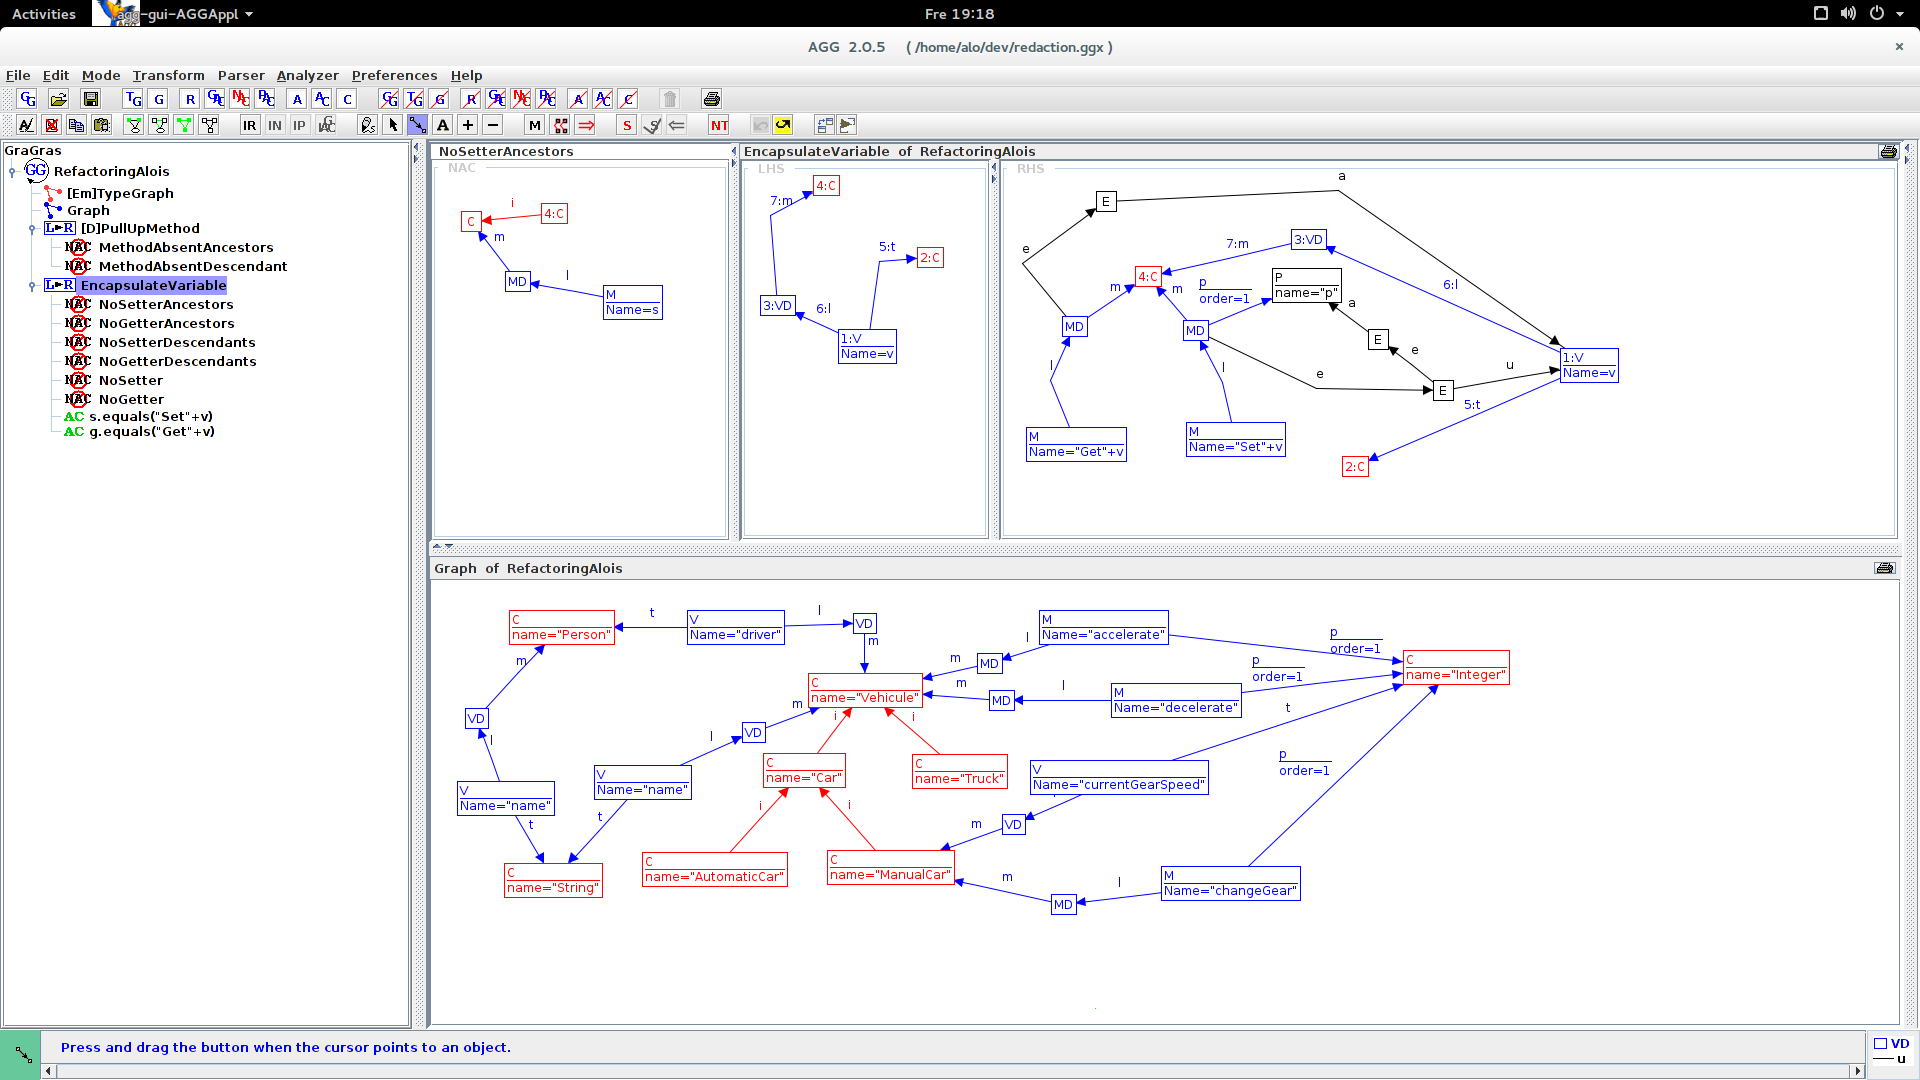
\includegraphics[width=\textwidth]{beforeEncapsulateVariable.png}
\end{myfig}

En haut de l'image~\ref{beforeEncapsulateVariable} se trouve la LHS qui représente la structure d'un sous graph du programme avant sa transformation. A droite, nous avons RHS qui représente la structure de ce sous graph après la transformation. Et en dessous nous avons le graphique du programme.

\begin{myfig}{afterEncapsulateVariable}{After Encapsulate Variable}
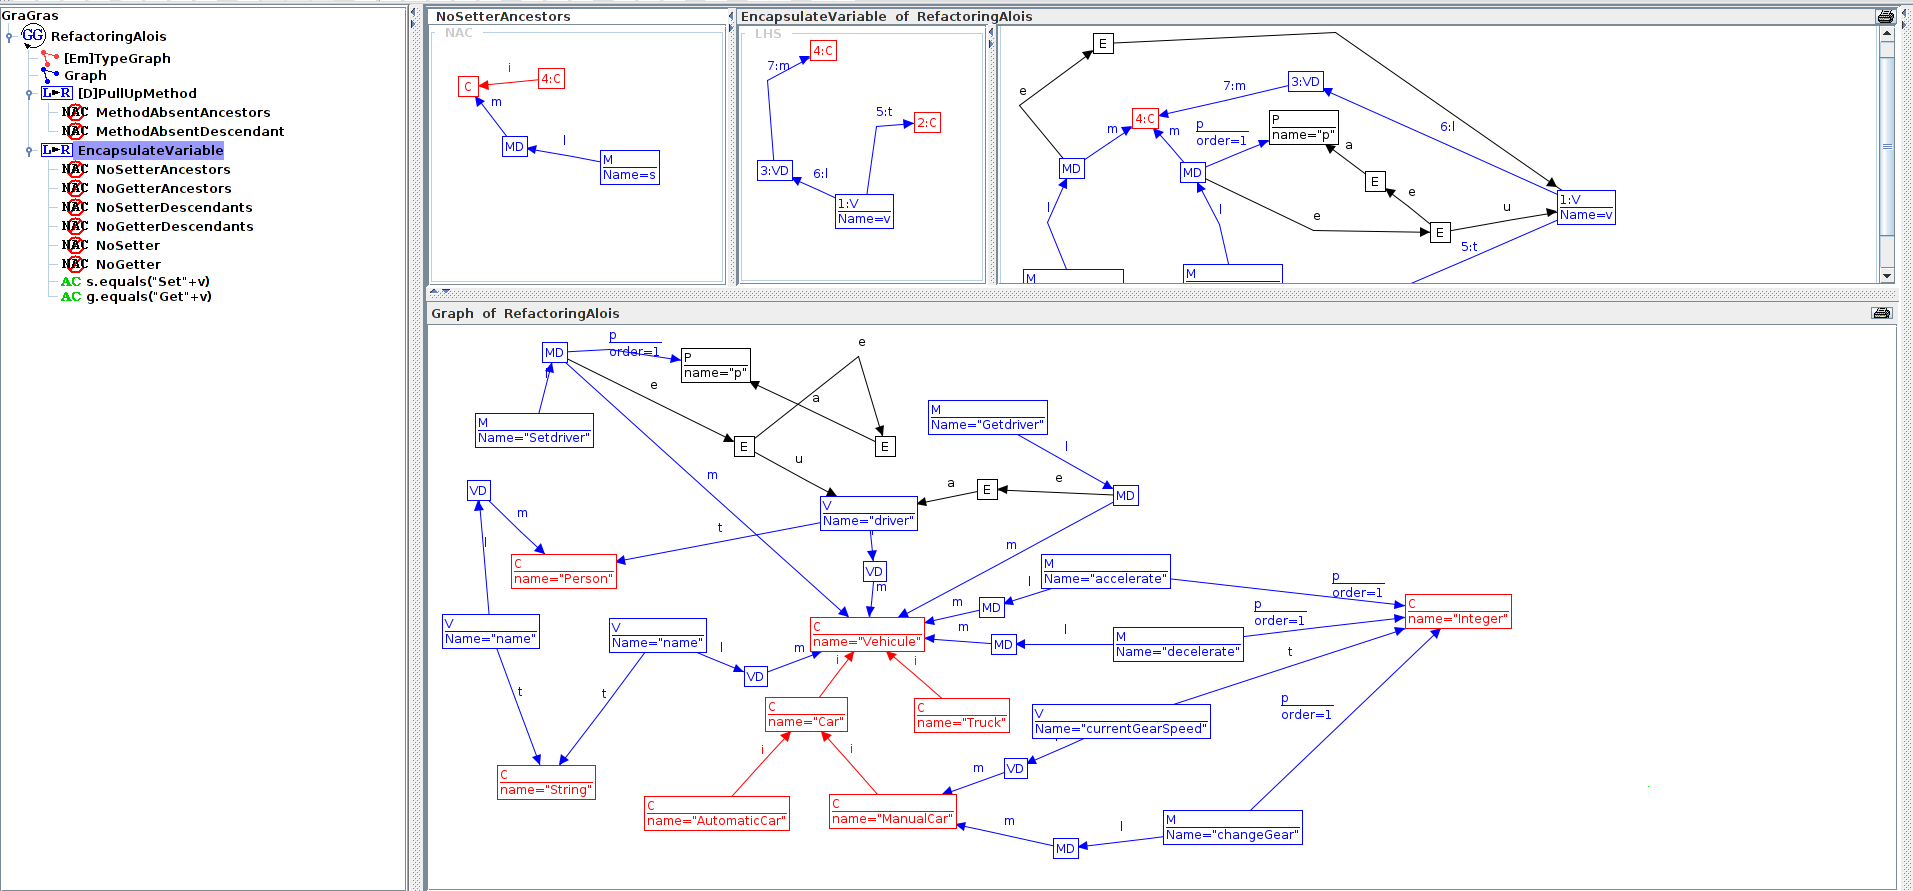
\includegraphics[width=\textwidth]{afterEncapsulateVariable.png}
\end{myfig}

Ici dans l'image~\ref{afterEncapsulateVariable} nous avons les mêmes éléments au dessus mais la partie inférieur à changer. 
Elle représente le graphique après l'application de la transformation.

Je n'ai laisser que la transformation du sous graph lié à la variable "driver" pour une meilleure visibilité. 

Normalement cette transformation s'applique à tout les sous graphs correspondant ce qui ici correspond à toute les variables membre d'une classe.

\subsection{Pull Up Method}

Cela Consiste à déplacer une méthode présente dans une ou plusieur classes enfant et l'insérer dans la classe parent.

\subsubsection{Example}

before :
\begin{lstlisting}[frame=single]
public class Vehicule {
	public String name;
	public Person driver;

        public void accelerating(int amount) { 
	}

	public void decelerate(int amount) { 
	}
}

public class Car extends Vehicule {

}

public class ManualCar extends Car {
	public void changeGear(int speed){ }
}
\end{lstlisting}

after :
\begin{lstlisting}[frame=single]
public class Vehicule {
	public String name;
	public Person driver;

	public void accelerating(int amount) {

	}
	public void decelerate(int amount) { 
	}

        public void changeGear(int speed){
	}
}

public class Car extends Vehicule {

}

public class ManualCar extends Car {

}
\end{lstlisting}
\subsubsection{Condition}
Les conditions sont:

- La classe parent ne peut pas déjà contenir une méthode ayant le même nom
- Aucune des variables directement accédée ou modifiée par la méthode ne peut être en dehors du scope de la classe parent.

WF-1 est préserver car on ne crée ni ne bougeons aucune variable.
WF-2 est préserver grâce à la précondition qui stipule qu'il ne peut pas se trouver une méthode avec la même signature dans la classe parent.
WF-3 est préservée grâce à la précondition qui stipule que la définition de la méthode bougée ne doit pas accéder à des variables en dehors du scope du parent.
WF-4 est préservée car on ne crée ni ne modifie aucune méthode.

\subsubsection{Représentation graphique}

\begin{myfig}{beforePullUpMethode}{Before PullUp Methode}
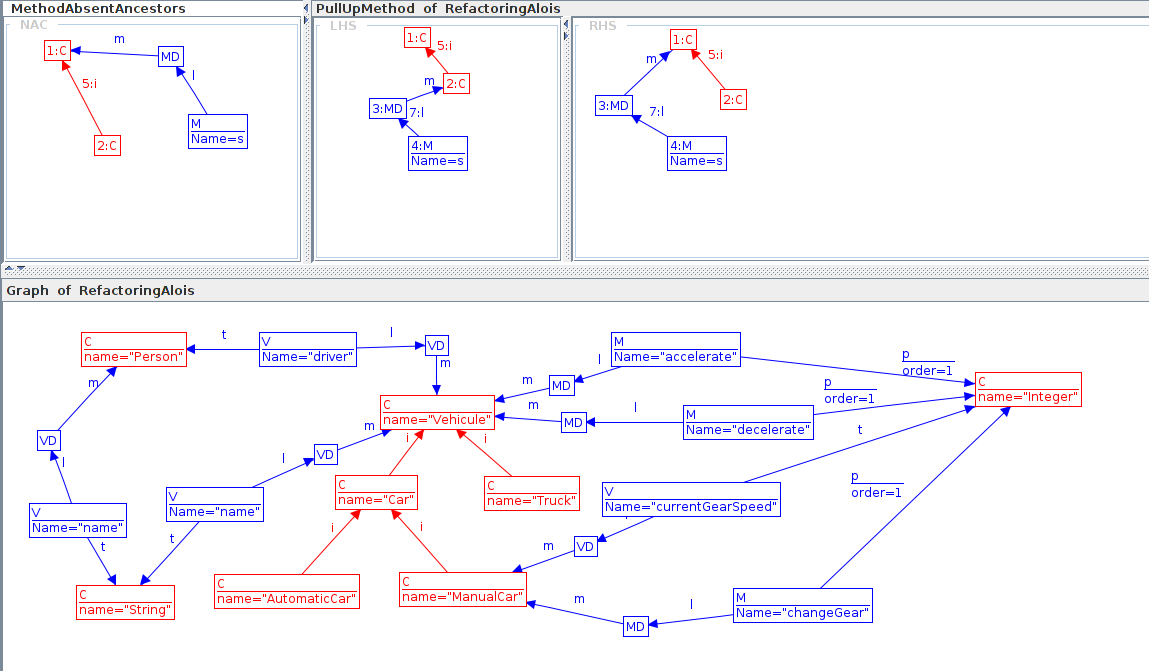
\includegraphics[width=\textwidth]{beforePullUpMethode.png}
\end{myfig}

En haut de l'image~\ref{beforePullUpMethode} se trouve la LHS qui représente la structure d'un sous graph du programme avant sa transformation. A droite, nous avons RHS qui représente la structure de ce sous graph après la transformation. Et en dessous nous avons le graphique du programme.

\begin{myfig}{afterPullUpMethod}{After PullUp Methode}
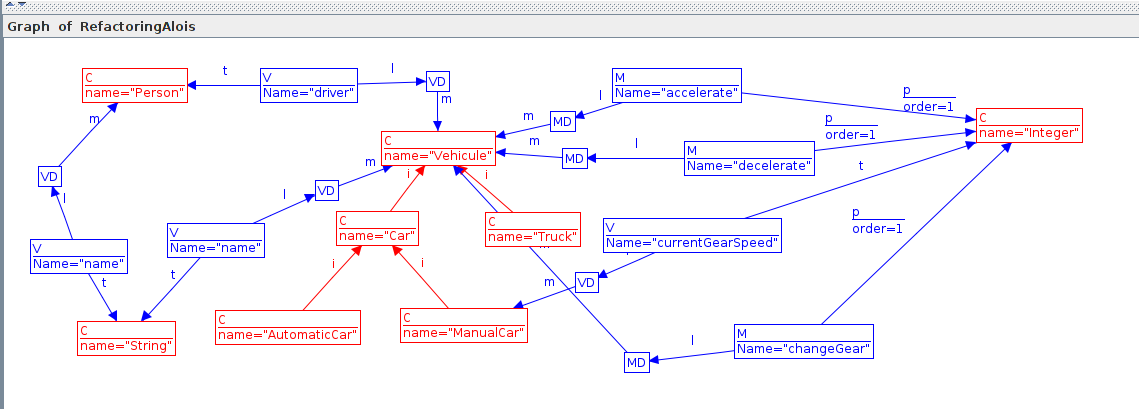
\includegraphics[width=\textwidth]{afterPullUpMethod.png}
\end{myfig}

Dans~\ref{afterPullUpMethod} la partie du dessous à changé et représente le programme après avoir appliqué la transformation en d'autre termes, après avoir
remonté la méthode de la classe ManualCar à Vehicule. Cette méthode est bien supprimée de la classe ManualCar car il n'existe plus de lien
vers celle çi.

\section{Préservation du comportement}

Nous avons définit au début que notre but était de prouver que les refactoring n'altérait pas le comportement d'un programme. Pour cela nous allons prouvez que certaines propriétés sont preservée après un refactoring. Et plus particulièrement les propriété de types, accès, mise à jour et appelle de méthode.

Il faut donc prouver que si l'on a une expression de graph avant la transformation, il doit exister la même ou une equivalence après cette transformation.

Pour cela nous aurons besoin d'une fonction de tracking appelée tr. Si G derive H utilisant un production P alors tr est une fonctient de Vg (set d nodes de G) dans Vh (set de nodes de H)

\subsection{Preservation d'un expression de graph}
GE, une expression de graph et G et H des graph de programme. La fonction tr: Vg -> Vh correspondance de node. Alors la fonction tr preserve GE si pour chaque occurance OC de GE dans G, tr x OC est une occurence de GE dans H.

Par example :

Montrer que une variable dans LHS X la fonction encapsulate => le getter , setter et la variable dans RHS

\subsection{Fonction de tracking}



\end{document}
